%%%%%%%% ICML 2019 EXAMPLE LATEX SUBMISSION FILE %%%%%%%%%%%%%%%%%

\documentclass{article}

%%%%%%%%%%%%%%%%%%%%%%%%%%%%%%%%%%%%%%%%%%%%%%%%%%%%%%%%%%%%%%%%%%%%%%%%%%%%%%%%
%       Packages added by Pablo in order to have nice math symbols             %
%%%%%%%%%%%%%%%%%%%%%%%%%%%%%%%%%%%%%%%%%%%%%%%%%%%%%%%%%%%%%%%%%%%%%%%%%%%%%%%%
\usepackage{amsmath}
\usepackage{subfig}
\usepackage{algorithm2e}
\usepackage{bm}
\usepackage{booktabs}
\usepackage{hyperref} % for \url{}
%\usepackage[justification=centering]{caption}

\usepackage{stmaryrd} % for \llbrackets
\usepackage{amsthm}  % for proof
\usepackage{IEEEtrantools} %because I like it
\usepackage{dsfont} % for unity matrix

\usepackage{mathtools} % For \triangleq
\usepackage{amssymb} % for \triangleq

\newtheorem{definition}{Definition}
\newtheorem{lem}{Lemma}
\newtheorem{theorem}{Theorem}



\usepackage[T1]{fontenc} % <- for italic non-serif F


\DeclareMathAlphabet{\mathsfit}{\encodingdefault}{\sfdefault}{m}{sl}
\SetMathAlphabet{\mathsfit}{bold}{\encodingdefault}{\sfdefault}{bx}{sl}


\newcommand{\mat}[1]{\bm{\mathsfit{#1}}}
\newcommand{\vect}[1]{\ensuremath{\boldsymbol{#1}}}

\newcommand{\Id}[1]{\bm{\mathsfit{I}}^{#1}_{\bm{\mathsfit{d}} }}
%\newcommand{\Id}[1]{\boldsymbol{\mathbb{I #1}}}

\newcommand{\vectone}[1]{\boldsymbol{\mathfrak{1 #1}}}


% Recommended, but optional, packages for figures and better typesetting:
\usepackage{microtype}
\usepackage{graphicx}
\usepackage{subfigure}
\usepackage{booktabs} % for professional tables

% hyperref makes hyperlinks in the resulting PDF.
% If your build breaks (sometimes temporarily if a hyperlink spans a page)
% please comment out the following usepackage line and replace
% \usepackage{icml2019} with \usepackage[nohyperref]{icml2019} above.
\usepackage{hyperref}

% Attempt to make hyperref and algorithmic work together better:
\newcommand{\theHalgorithm}{\arabic{algorithm}}

% Use the following line for the initial blind version submitted for review:
\usepackage{icml2019}

% If accepted, instead use the following line for the camera-ready submission:
%\usepackage[accepted]{icml2019}

% The \icmltitle you define below is probably too long as a header.
% Therefore, a short form for the running title is supplied here:
\icmltitlerunning{Rational Matrix Machines}

\begin{document}

\twocolumn[
\icmltitle{Rational Matrix Machines \\ \normalsize{\textit{a general algorithm for learning complex rational matrix functions} }}

% It is OKAY to include author information, even for blind
% submissions: the style file will automatically remove it for you
% unless you've provided the [accepted] option to the icml2019
% package.

% List of affiliations: The first argument should be a (short)
% identifier you will use later to specify author affiliations
% Academic affiliations should list Department, University, City, Region, Country
% Industry affiliations should list Company, City, Region, Country

% You can specify symbols, otherwise they are numbered in order.
% Ideally, you should not use this facility. Affiliations will be numbered
% in order of appearance and this is the preferred way.
\icmlsetsymbol{equal}{*}

\begin{icmlauthorlist}
\icmlauthor{Pablo Ducru}{equal,to}
\icmlauthor{Vladimir Sobes}{equal,to,goo}
% \icmlauthor{Cieua Vvvvv}{goo}
% \icmlauthor{Iaesut Saoeu}{ed}
% \icmlauthor{Fiuea Rrrr}{to}
% \icmlauthor{Tateu H.~Yasehe}{ed,to,goo}
% \icmlauthor{Aaoeu Iasoh}{goo}
% \icmlauthor{Buiui Eueu}{ed}
% \icmlauthor{Aeuia Zzzz}{ed}
% \icmlauthor{Bieea C.~Yyyy}{to,goo}
% \icmlauthor{Teoau Xxxx}{ed}
% \icmlauthor{Eee Pppp}{ed}
\end{icmlauthorlist}

\icmlaffiliation{to}{Massachusetts Institute of Technology, Center for Computational Engineering and Department of Nuclear Science and Engineering | Tsinghua University, Schwarzman Scholars.}
\icmlaffiliation{goo}{Oak Ridge National Laboratory | University of Tennessee, Knoxville, TN, USA.}
\icmlaffiliation{ed}{Department of Nuclear Science \& Engineering, Massachusetts Institute of Technology, Cambridge, MA, U.S.A.}

\icmlcorrespondingauthor{Pablo Ducru}{p_ducru@mit.edu}

% You may provide any keywords that you
% find helpful for describing your paper; these are used to populate
% the "keywords" metadata in the PDF but will not be shown in the document
\icmlkeywords{Rational Matrix Machines, complex shallow networks, rational approximation, complex rational matrix functions, vector fitting}

\vskip 0.3in
]

% this must go after the closing bracket ] following \twocolumn[ ...

% This command actually creates the footnote in the first column
% listing the affiliations and the copyright notice.
% The command takes one argument, which is text to display at the start of the footnote.
% The \icmlEqualContribution command is standard text for equal contribution.
% Remove it (just {}) if you do not need this facility.

%\printAffiliationsAndNotice{}  % leave blank if no need to mention equal contribution
\printAffiliationsAndNotice{\icmlEqualContribution} % otherwise use the standard text.


\begin{abstract}
%This document provides a basic paper template and submission guidelines.
%Abstracts must be a single paragraph, ideally between 4--6 sentences long.
%Gross violations will trigger corrections at the camera-ready phase.




Inferring the rational function that best fits a set of observed outputs at given points is a centuries old problem.
Physics often generates resonant phenomena whose mathematical forms are rational functions. 
They thus appear in myriad systems, from quantum scattering and spectroscopy, to multi-input multi-output (MIMO) transfer functions of coupled linear differential equations in electrical engineering. 
Because rational functions exhibit both a strong local behavior and a long-range tail effect, they are also used for universal approximation. 
Since Pad\'e approximants, traditional methods have focused on the polynomials ratio approach, $\mat{F}(z)  \triangleq \frac{\sum_{n=0}^{N_n}\mat{A_n}z^n}{\sum_{n=0}^{N_d} b_n z^n}$, and requires to pre-specify the degrees of the numerator and denominator $N_n$, $N_d$. These methods have been extensively used in physics, electrical engineering, or signal processing.

In this article, we look at this old problem of rational approximation from a novel statistical learning theory perspective. From the partial fraction decomposition form, $\mat{F}(z) \triangleq \sum_{n=0}^{N_p} \frac{\mat{R_n}}{z-p_n} + \mat{C}$, learning these resonances is akin to a one-layer neural network, where the features (or atoms) $\varphi_{n}(z) \triangleq \frac{1}{z-p_n}$ are determined by the poles $\left\{ p_n \right\}$, and the linear combination coefficients are the residues $\big\{ \mat{R_n}\big\}$: we call this a \textit{Rational Matrix Machine}.

Training a Rational Matrix Machine (RMM) requires performing both feature extraction (finding the poles $\left\{ p_n \right\}$) and feature selection (finding the residues $\big\{ \mat{R_n}\big\}$). The former is a highly non-linear process for which current Machine Learning (ML) methods are inadequate. 


% on these Rational Matrix Machines, we here establish a universal method for rational approximation of complex matrix-valued functions without the need to pre-specify the degrees of the approximation.


We here derive a general algorithm to train Rational Matrix Machines (RMM) in a supervised way: given a set of complex points and associated complex matrices $\Big\{ z_k , \mat{Y_k} \Big\}$ our RMM algorithm learns the complex poles $\left\{ p_n \right\}$ and matrix residues $\big\{ \mat{R_n}\big\}$ of the best approximate complex matrix-valued rational function $\mat{F}(z)$, without the need to pre-specify the degrees of the approximation. 
This establishes a universal ML algorithm for rational functions Hilbert spaces. 

Tested on experimental observations of Oxygen-16 nuclear cross sections, our RMM algorithm was able to learn the physical radioactive parameters of the scattering matrix, and match the results predicted by the R-matrix theory of quantum nuclear interactions. This is the first evidence of a ML algorithm learning nuclear resonances. 









% Inferring the rational functions that have generated a set of observed resonances is the centuries-old problem of rational approximation.


% Also, Physics often generates resonant phenomena whose mathematical forms are rational functions. 
% Rational functions thus appear in myriad physical and engineering systems governed by resonance behavior: from quantum scattering and spectroscopy, to multi-input multi-output transfer functions of coupled linear differential equations in electrical engineering. 
% Inferring the rational functions that have generated a set of observed resonances is the centuries-old problem of rational approximation.
\end{abstract}


%============================================================================
%||||||||||||||||||||||||||||||||||||||||||||||||||||||||||||||||||||||||||||
\section{\label{Introduction}Introduction -- rational matrix functions}
%||||||||||||||||||||||||||||||||||||||||||||||||||||||||||||||||||||||||||||
%============================================================================

\IEEEPARstart{D}{eep} networks have been at the forefront of the monumental progress in machine learning (ML) and artificial intelligence (AI) witnessed in the past decade. However, shallow networks still have their say when addressing certain types of problems.
One such one-layer network is formed of rational functions.

Physics often dictates rational functions. Myriad problems give rise to resonant behavior: from transfer functions of coupled linear differential equations in electrical engineering, to physical resonances of quantum scattering interactions in spectroscopy, resonances are intrinsically characterized by a linear combination of complex poles and residues.

Modeling of resonant behavior therefore requires learning rational functions from noisy experimental data: provided a set of observed complex points and associated complex matrices $\Big\{ z_k \, , \, \mat{Y_k} \Big\} \in \Big\{  \mathbb{C} \times  \mathbb{C}^{h\times q} \Big\}_{k\in \llbracket 1 , N_k \rrbracket}  $, we must search the Hilbert space of rational functions to infer the one rational function $\mat{F}(z) $ most likely to have generated the data.


Rational functions are universal approximators (c.f. Runge's 1885 theorem), and rational approximation is a century-old field, pioneered by Heni Pad\'e, which has greatly expanded and been abundantly deployed over the years, either because the form of the problem requires a rational solution, or because of the superior characteristics of rational functions, specially their localized and long-tail evanescence properties over polynomial fitting. For instance ``pole-zero modeling'' has been central to electrical engineering and signal processing. These traditional rational approximation approaches all focus either on the coefficients of the numerator and denominator, or on its poles and roots (and sometimes on continued fractions) [CITE: PADE APPOXIMATION, REMEZ ALGORITHM, SK ITERATION]:
\begin{equation}
\begin{IEEEeqnarraybox}[][c]{C}
\IEEEstrut
 \mat{F}(z) = \frac{\sum_{n=1}^{N_n} \mat{A_n} z^n}{\sum_{n=1}^{N_p} b_n z^n}  \quad,  \quad \mat{F}(z) = \frac{\bigcirc_{n=1}^{N_n} \left(\mat{\alpha_n} - z \vectone{} \otimes \vectone{} \right) }{\prod_{n=1}^{N_p} (z-p_n)} 
\end{IEEEeqnarraybox}
\label{eq:: traditional rational approximation}
\end{equation}
where $\circ$ designates the element-wise Hadamard product, $\otimes$ the tensor product, and $\vectone{} \triangleq \left[ 1, 1, \hdots, 1 \right]^\mathsf{T}$ is the vector composed of ones. \\

We here focus on the Hilbert space $\mathcal{F}$ of proper rational matrix functions, i.e. without entire polynomial part other than an offset: $\mathcal{F} = \Big\{ \mat{F}: \mathbb{C} \mapsto \mathbb{C}^{h\times q}  , \;  \mat{F}(z) \text{ from (\ref{eq:: traditional rational approximation})} \; \big| \; N_n \leq N_p  \Big\}$. %$\mathcal{F} = \Big\{ \mat{F}: \mathbb{C} \mapsto \mathbb{C}^{h\times q}  \; , \;   \mat{F}(z) \triangleq \frac{\sum_{n=1}^{N_n} \mat{A_n} z^n}{\sum_{n=1}^{N_p} b_n z^n} \; \; \big| \; \; N_n \leq N_p  \Big\}$.
Using the traditional $\mathrm{L_2}$ norm for regression, solving the rational approximation problem would minimize the distance between the functions in the $\mathcal{F}$ space of rational functions:

\begin{equation}
\begin{IEEEeqnarraybox}[][c]{C}
\IEEEstrut
\underset{\mat{F} \in \mathcal{F}}{\mathrm{min}} \; \mathcal{E}\left[\mat{F}\right] \\ \mathcal{E}\left[\mat{F}\right]   \ \triangleq \  \int_{z\in\mathbb{C}}  \left\| \mat{F}(z) - \mat{Y}(z) \right\|_{\mathrm{L}_2}^2 \mathrm{d}\rho(z)
\end{IEEEeqnarraybox}
\label{problem:: theoretical rational approximation problem}
\end{equation}

In practice, provided observed data points $\big\{z_k, \mat{Y_k}\big\}_{k\in\llbracket 1, N_k \rrbracket}$ with weights $\big\{\rho_k\big\}_{k\in\llbracket 1, N_k \rrbracket}$ (so that $\sum_{k=1}^{N_k}\rho_k = 1$), solving the rational approximation problem means minimizing the regularized  empirical weighted least square error $\widehat{\mathcal{E}}_\lambda$:

\begin{equation}
\begin{IEEEeqnarraybox}[][c]{C}
\IEEEstrut
\underset{\mat{F} \in \mathcal{F}}{\mathrm{min}} \; \widehat{\mathcal{E}}_\lambda \left[\mat{F}\right]  \\  \widehat{\mathcal{E}}_\lambda\left[\mat{F}\right]   \ \triangleq \  \sum_{k=1}^{N_k} \rho_k \left\| \mat{F}(z_k) - \mat{Y_k} \right\|_{\mathrm{L}_2}^2 +  \mathcal{R}_\lambda \left[\mat{F}\right]
\end{IEEEeqnarraybox}
\label{problem:: rational approximation weighted least squares plus regularization}
\end{equation}
where $ \mathcal{R}_\lambda \left[\mat{F}\right]$ is a regularization term aimed at compensating the over-fitting tendency of the pure least-squares problem:
\begin{equation}
\begin{IEEEeqnarraybox}[][c]{C}
\IEEEstrut
\underset{\mat{F} \in \mathcal{F}}{\mathrm{min}} \; \widehat{\mathcal{E}}\left[\mat{F}\right]    \\  \widehat{\mathcal{E}}\left[\mat{F}\right]  \ \triangleq \  \sum_{k=1}^{N_k} \rho_k \left\| \mat{F}(z_k) - \mat{Y_k} \right\|_{\mathrm{L}_2}^2
\end{IEEEeqnarraybox}
\label{problem:: rational approximation weighted least squares}
\end{equation}
Even the latter purely quadratic optimization problem on complex functions is difficult because it is highly non-linear, non-convex, and ill-conditioned. Moreover, the number of poles $N_p \in \mathbb{N}$ (degree of the denominator) is \textit{a priori} unspecified. Yet, previous methods -- such as Pad\'e approximation -- require to specify explicitly the degrees of both $N_n$ and $N_p$, in essence limiting the search to a sub-space of $\mathcal{F}$.


%============================================================================
%||||||||||||||||||||||||||||||||||||||||||||||||||||||||||||||||||||||||||||
\section{\label{sec: Rational Matrix Machines}Rational Matrix Machines}
%||||||||||||||||||||||||||||||||||||||||||||||||||||||||||||||||||||||||||||
%============================================================================


In this article, we look at this old problem of rational approximation from a novel statistical learning theory viewpoint. Focusing on proper rational functions $\mat{F} \in \mathcal{F}$, where $N_n \leq N_p$, we take the partial fraction decomposition: 
\begin{equation}
\begin{IEEEeqnarraybox}[][c]{C}
\IEEEstrut
 \mat{F}(z) \triangleq \sum_{n=0}^{N_p} \frac{\mat{R_n}}{z-p_n} + \mat{C}
\end{IEEEeqnarraybox}
\label{eq:: partial fraction rational approximation}
\end{equation}
The rational matrix function $\mat{F}(z)$ is then akin to a one-layer neural network, where the features (or atoms) $\varphi_n(z)$ are uniquely determined by the poles $\big\{ p_n \big\}$, and the linear combination coefficients are the residues $\big\{ \mat{R_n} \big\}$: 
\begin{equation}
\begin{IEEEeqnarraybox}[][c]{C}
\IEEEstrut
 \mat{F}(z) = \sum_{n=1}^{N_p} \mat{R_n} \; \varphi_{n}(z)  + \mat{C} \quad, \quad \varphi_{n}(z) \triangleq \frac{1}{z-p_n}
\end{IEEEeqnarraybox}
\label{eq:: def of Rational Matrix Machine}
\end{equation}
we shall henceforth call this a \textit{Rational Matrix Machine}.

Mathematically, there is no difference between the Rational Matrix Machine (\ref{eq:: def of Rational Matrix Machine}) and traditional rational approximations (\ref{eq:: traditional rational approximation}). However, they differ in both spirit and form.
In form, the Rational Matrix Machine linear combination of features (\ref{eq:: def of Rational Matrix Machine}) isolates the individual contributions of each resonance, which is often much more convenient for subsequent treatment. 
In spirit, Rational Matrix Machines portray regression  (\ref{problem:: rational approximation weighted least squares plus regularization}) as a machine learning problem: solving (\ref{problem:: rational approximation weighted least squares plus regularization}) means training the Rational Matrix Machine (\ref{eq:: def of Rational Matrix Machine}).
This brings useful statistical learning theory concepts -- such as Reproductive Kernel Hilbert Spaces (RKHS) and regularization -- to address this centuries-old problem. 


Training a Rational Matrix Machine is not straightforward: both feature extraction -- learning the number $N_p$ and set of poles $\big\{ p_n \big\}_{n \in \llbracket 1, N_p \rrbracket}$ -- and feature selection -- learning the corresponding residues $\big\{ \mat{R_n} \big\}_{n \in \llbracket 1, N_p \rrbracket}$ and the offset $\mat{C}$ -- must be performed.
Moreover, poles introduce highly non-linear (actually resonant) behavior that impeach resorting to traditional gradient-descent methods for the feature extraction.
Thankfully, significant progress has been achieved to converge the poles $\big\{ p_n \big\}$ in the case where their number $N_p$ is fixed: in 2006 Gustavsen implemented a very successful Sanathanan-Koerner iteration by barycentric pole relocation (BPR), giving birth to the now widespread Vector Fitting (VF) algorithm [CITE]. 
Regarding how to learn the number of poles $N_p$, problem-specific \textit{ad-hoc} approaches have been proposed to filter out spurious poles [CITE pole trimming], though the authors are unaware of any systematic and general method.

%============================================================================
%||||||||||||||||||||||||||||||||||||||||||||||||||||||||||||||||||||||||||||
\section{\label{sec: Training Rational Matrix Machines}Training Rational Matrix Machines}
%||||||||||||||||||||||||||||||||||||||||||||||||||||||||||||||||||||||||||||
%============================================================================

In this article, we build upon these past achievements to establish a universal ML algorithm to train Rational Matrix Machines (RMM). We break down the feature extraction process into iterations of pole convergence -- performed with barycentric pole relocation (BPR) -- and pole filtering -- performed with a new group-$\mathrm{L_1}$-$\mathrm{L_2}$ regularization on complex Frobenius norms we specially tailored to Rational Matrix Machines and which we managed to solve by generalizing the Proximal-Forward-Backward-Splitting (PFBS) algorithm to complex matrices. 
Once the features are extracted, the feature selection step becomes a classical regularized least-square problem. 

% NOTE: if RKHS, this means we can solve the residues retrieval problem in a data-driven, unsupervised manner ? 


%============================================================================
\subsection{\label{sec: Feature extraction}Feature extraction -- pole finding}
%============================================================================

The process of feature extraction consists of learning the set of poles $\big\{ p_n \big\}_{n \in \llbracket 1, N_p \rrbracket}$, including their number $N_p$.
To do so we take a ``kitchen sink'' approach whereby we start at $t_0$ with a large number of poles $N_p^{t_0} \gg N_p$, say $N_p^{t_0} = \mathrm{floor}\left[\frac{N_k}{3}\right]$ (it is impossible to infer a resonance from less than 3 points).\\
We then set-up the following iterative scheme to progressively diminish the estimated number of poles $N_p^t \geq N_p^{t+1} $ until we hopefully converge to the true value $N_p$.

%============================================================================
\subsubsection{\label{sec: Pole convergence}Pole convergence}
For this feature-extraction step, we fix the number of poles $N_p^t$ and search corresponding poles $\big\{ p_n \big\}_{n \in \llbracket 1, N_p^t \rrbracket}$ using barycentric pole relocation (BPR). 

Finding the poles $\big\{ p_n \big\}_{n \in \llbracket 1, N_p^t \rrbracket}$ in (\ref{problem:: rational approximation weighted least squares}) is a highly non-linear problem. BPR elegantly overcomes this by decomposing it into two standard linear-algebra problems, and iterating over until the poles converge.
Rather than solving problem (\ref{problem:: rational approximation weighted least squares}) directly, BPR starts with some initial poles guess $\big\{ p_n^{i_0} \big\}_{n \in \llbracket 1, N_p^t \rrbracket}$, and for each iteration $i$ solves the Sanathanan-Koerner (SK) problem:

\begin{equation}
\begin{IEEEeqnarraybox}[][c]{C}
\IEEEstrut
\mathrm{min} \ \widehat{\mathcal{E}}_{\mathrm{SK}}^{i} \quad , \quad \widehat{\mathcal{E}}_{\mathrm{SK}}^{i}  \ \triangleq \  \sum_{k=1}^{N_k} \rho_k \left\| \mat{F}^{i}(z_k) - b^{i}(z_k) \mat{Y_k}  \right\|_{\mathrm{L}_2}^2
\end{IEEEeqnarraybox}
\label{Problem: iteration i SK problem}
\end{equation}
in such a way that the introduced barycentric function $b^{i}(z)$ goes to one as we iterate ($b^{i}(z) \underset{i \rightarrow \infty}{\longrightarrow} 1$), so that we end-up solving the initial problem (\ref{problem:: rational approximation weighted least squares}).
Each pole convergence iteration $i$ is then a two-step process:

\begin{enumerate}
  \item \textbf{Barycentric residue selection:}. The barycentric function $b^{i}(z)$ is defined as
    \begin{equation}
    \begin{IEEEeqnarraybox}[][c]{rCl}
    \IEEEstrut
    b^{i}(z)& \triangleq & 1 + \sum_{n=1}^{N_p} \frac{r_n^{i+1}}{z-p_n^{i}} 
    \end{IEEEeqnarraybox}
    \label{eq: baricentric function b pole expansion}
    \end{equation}
which crucially shares the same poles as the rational matrix function at iteration $i$: $\mat{F}^{i}(z)  \triangleq \sum_{n=1}^{N_p} \frac{\mat{R_n}^{i}}{z-p_n^{i}} + \mat{C}^{i} $. We here fix the poles $\left\{p_n^{i}\right\}_{n\in \llbracket 1 , N_p^t \rrbracket}$ and find the barycentric residues $\left\{r_n^{i+1}\right\}_{n\in \llbracket 1 , N_p^t \rrbracket}$ by solving the now quadratic least-squares problem (\ref{Problem: iteration i SK problem}).

PABLO: HERE, WE COULD PROPOSE AN ALL IN ONE BARYCENTRIC RESIDUES SELECTION WHERE INSTEAD OF SOLVING $\widehat{\mathcal{E}}\left[\mat{F}\right] $ FROM (\ref{Problem: iteration i SK problem}), WE COULD SOLVE $\widehat{\mathcal{E}}^{\mathrm{PF}}_\lambda \left[\mat{F}\right] $ FROM (\ref{problem:: Pole Filtering}) WITH THE PFBS. NO IDEA HOW THIS WILL BEHAVE, THOUGH IT WOULD BE QUITE ELEGANT IF IT BOTH FINDS THE RIGHT POLES AND THE RIGHT NUMBER OF POLES ALL IN ONE !
AND, IT WOULD MAKE THE ENTIRE ALGORITHM MUCH SHORTER. 
AND, WE COULD FOCUS ON THE $r_n$ ONLY IN THE PFBS DESCENT 5NOT REALLY TRUE, AS WE NEED TO UPDATE THE $\mat{R_n}$ TOO, SPECIALLY THE gRADIENT ON THE $r_n$ IS INDEPENDENT ON THE PENALIZAITON, SO NO PROBLEM OF SOLVING THE ENTIRE MATIRIX ! AND, ONCE WE BELIEVE WE'VE CONVERGED THE POLES, WE CAN STILL SWITCH TO A TICHONOCV REGULARIZATION IF WE THINK IT IS WORTH-WILE. 
THIS OPERATION COULD BE CALLED BARYCENTRIC RESIDUES FILTERING. 
OF COURSE, WE COULD HAVE A PROGRESSIVE PENALIZATION AS THE POLES CONVERGE, TO HELP THIS STABILIZE A BIT. 
NO IDEA HOW THIS WILL WORK, IF AT ALL. BUT IT MIGHT BE MORE STABLE THAN THE STANDARD VF !


  \item \textbf{Barycentric pole relocation:} with these newfound residues $\left\{r_n^{i+1}\right\}_{n\in \llbracket 1 , N_p^t \rrbracket}$, we define the new the poles $\left\{p_n^{i+1}\right\}_{n\in \llbracket 1 , N_p^t \rrbracket}$ as the roots of the barycentric function $b^i(z)$. That is we solve $b^i(z) = 0 $, and update the poles as:

\begin{equation}
\begin{IEEEeqnarraybox}[][c]{rCl}
b^{i}(z)& = &  \frac{\prod_{n=1}^{N_p}\left( z-p_n^{i+1} \right)}{\prod_{n=1}^{N_p}\left( z-p_n^{i} \right)}
\IEEEstrut\end{IEEEeqnarraybox}
\label{eq: baricentric function b pole factorized}
\end{equation}

As poles converge, we have $b^{i} \underset{i\rightarrow \infty}{\longrightarrow} 1$, entailing we solve the initially intended minimization (\ref{problem:: rational approximation weighted least squares}). 

To find the next-iteration poles $\left\{p_n^{i+1}\right\}_{n\in \llbracket 1 , N_p^t \rrbracket}$ in (\ref{eq: baricentric function b pole factorized}), we can show that finding the roots of $b^i(z) = 0 $ is equivalent to finding the eigenvalues of the matrix $\mat{Diag}\left[ p_n^{i}\right] - \boldsymbol{r}^{i+1}\otimes\boldsymbol{1}_{n}^\mathsf{T}$, that is
\begin{equation}
\begin{IEEEeqnarraybox}[][c]{C}
\IEEEstrut
 \Big\{p_n^{i+1}\Big\}_{n\in \llbracket 1 , N_p \rrbracket} = \mathcal{S}_p\Big(\mat{Diag}\left[ p_n^{i}\right] - \boldsymbol{r}^{i+1}\otimes\boldsymbol{1}_{n}^\mathsf{T} \Big)  
\end{IEEEeqnarraybox}
\label{Problem: eigenvalue pole update}
\end{equation}
 where $\mathcal{S}_p\big(\cdot\big)$ calls the spectrum (eigenvalues), $\mat{Diag}\left[ p_n^{i}\right]$ is the diagonal matrix of the $i$-th iteration poles, $\boldsymbol{1}_{n} $ is the $N_p$-length vector of ones $\boldsymbol{1}_{n} = \left[ 1, \hdots , 1 \right]^\mathsf{T}$, and $\boldsymbol{r}^{i+1} = \left[ r_1^{i+1}, \hdots , r_{N_p}^{i+1} \right]^\mathsf{T}$ is the $N_p$-length vector of residues of barycentric function $b^{i}(z)$. 
 
\end{enumerate}

This is Gustaven's crucial improvement upon traditional SK iterations, which is at the core of the VF algorithm: it is fast, stable, and at convergence guarantees $b^{i}(z) \underset{i \rightarrow \infty}{\longrightarrow} 1$, though poles convergence is not guaranteed (cf. \cite{Drmac_2014}, section 2.1).


Each pole convergence iteration $i$ thus consists of computing $\left\{r_n^{i+1}\right\}_{n\in \llbracket 1 , N_p^t \rrbracket}$ in (\ref{eq: baricentric function b pole expansion}) -- by solving (\ref{Problem: iteration i SK problem}) with fixed poles $\left\{p_n^{i}\right\}_{n\in \llbracket 1 , N_p^t \rrbracket}$  -- and then computing updated poles $\left\{p_n^{i+1}\right\}_{n\in \llbracket 1 , N_p^t \rrbracket}$ in (\ref{eq: baricentric function b pole factorized}) -- by solving (\ref{Problem: eigenvalue pole update}). This is repeated until poles converge (in practice, tens of $i$ iterations suffice). 



% NOTE: QR (big memory imporvement), and relaxed (not certain in ti better), stability issues might be solved by pole filtering. 



%============================================================================
\subsubsection{\label{sec: Pole filtering}Pole Filtering}
Pole convergence fixed the number of poles $N_p^t$ and found corresponding poles $\big\{ p_n^{i} \big\}_{n \in \llbracket 1, N_p^t \rrbracket}$ (converged poles $p_n = p_n^{i_{\mathrm{end}}} $).
Pole filtering will now diminish the number of poles $N_p^t \geq N_p^{t+1}$ by filtering out the superfluous ones. 
Superfluous poles are identified as those which yield residues that are not robust to a small change in the data (that means these poles are the most likely to be over-fitting). 
We here find these non-robust residues by solving this new pole-filtering group regularization problem:

\begin{equation}
\begin{IEEEeqnarraybox}[][c]{C}
\IEEEstrut
\underset{\mat{R_n}, \mat{C} }{\mathrm{min}} \;  \widehat{\mathcal{E}}^{\mathrm{PF}}_\lambda \left[\mat{F}\right] \\  \widehat{\mathcal{E}}^{\mathrm{PF}}_\lambda \left[\mat{F}\right] \ \triangleq \  \sum_{k=1}^{N_k} \rho_k \left\| \mat{F}(z_k) - \mat{Y_k} \right\|_{\mathrm{L}_2}^2 +  \mathcal{P}_\lambda \left[\mat{R_n}\right] \\
\mathcal{P}_\lambda \left[\mat{R_n}\right]  \triangleq \lambda  \sum_{n=0}^{N_p} \frac{\left\| \mat{R_n}\right\|_{\mathrm{L_2}}}{\mathrm{min}_k \left|z_k-p_n\right|}
\end{IEEEeqnarraybox}
\label{problem:: Pole Filtering}
\end{equation}

Where $\mathrm{min}_k \left|z_k-p_n\right| \triangleq \underset{k\in \llbracket 1 , N_k \rrbracket}{\mathrm{min}} \left|z_k-p_n\right|$. 
This is a sparsity-inducing group-Lasso $\mathrm{L_1}$-$\mathrm{L_2}$ type of penalization we specially tailored to our complex rational matrix functions Hilbert space. $\left\|\cdot \right\|_{\mathrm{L_2}}$ is the Frobenius norm associated to the Hilbert-Schmidt hermitian product. 
Solving (\ref{problem:: Pole Filtering}) will drive some residue-matrices $\mat{R_n}$ to zero. We remove their corresponding poles $p_n$, so that $N_p^t \geq N_p^{t+1}$ and this constitutes a new $t \to t+1$ iteration. 
Once the number of poles has stabilized, we can consider the feature extraction process finished an proceed to feature selection. 

A major contribution of this article is the introduction of the pole-filtering problem (\ref{problem:: Pole Filtering}), which filters poles by identifying non-robust residues. We also provide an iterative means to solve (\ref{problem:: Pole Filtering}) in complex-matrix space by generalizing the Proximal Forward Backward Splitting Algorithm (PFBS) into the following pole filtering PFBS algorithm (PFA).
If (PFA) iterations 
\begin{equation}
\begin{IEEEeqnarraybox}[][c]{C}
\left[\begin{array}{c}
      \mat{R_n}^{\ell+1} \\
      \mat{C}^{\ell+1}
\end{array}\right] 
     = \left[ 
\begin{array}{c}
    \mathrm{prox}_{\mathcal{P}_\lambda}\Big( \mat{R_n}^{\ell} - \gamma \eth_{\mat{R_n}}\widehat{\mathcal{E}}\left[\mat{F}^\ell \right] \Big)\\
    \mat{C}^{\ell} -\gamma \eth_{\mat{C}}\widehat{\mathcal{E}}\left[\mat{F}^\ell \right]
\end{array} \right]
\IEEEstrut\end{IEEEeqnarraybox}
\label{theo::PFBS Pole Filtering}
\end{equation}
where 
\begin{equation}
\begin{IEEEeqnarraybox}[][c]{C}
    \mathrm{prox}_{\mathcal{P}_\lambda}\Big( \mat{R_n}^{\ell} - \gamma \eth_{\mat{R_n}}\widehat{\mathcal{E}}\left[\mat{F}^\ell \right] \Big)  =  \Big( \mat{R_n}^{\ell} - \gamma \eth_{\mat{R_n}}\widehat{\mathcal{E}}\left[\mat{F}^\ell \right] \Big)  \\ \times  \mathrm{max}\left\{ 0, 1 - \frac{\lambda / \mathrm{min}_k \left|z_k-p_n\right|}{\left\|\mat{R_n}^{\ell} - \gamma \eth_{\mat{R_n}}\widehat{\mathcal{E}}\left[\mat{F}^\ell\right] \right\|_{\mathrm{L_2}}} \right\}
\IEEEstrut\end{IEEEeqnarraybox}
     \label{theo:: Proximal for Pole Filtering}
\end{equation}

with
\begin{equation}
\begin{IEEEeqnarraybox}[][c]{C}
    \eth_{\mat{R_n}}\widehat{\mathcal{E}}\left[\mat{F}^\ell \right] =  \sum_{k=1}^{N_k} \frac{2 \rho_k }{z_k^*-p_n^*} \left[ \sum_{n=1}^{N_p} \frac{\mat{R_n}^{\ell}}{z_k-p_n} + \mat{C}^{\ell} - \mat{Y_k}  \right] 
\IEEEstrut\end{IEEEeqnarraybox}
\label{theo:: Cartesian gradient Rn expression}
\end{equation}
\begin{equation}
\begin{IEEEeqnarraybox}[][c]{C}
    \eth_{\mat{C}}\widehat{\mathcal{E}}\left[\mat{F}^\ell \right] =  \sum_{k=1}^{N_k} 2 \rho_k  \left[ \sum_{n=1}^{N_p} \frac{\mat{R_n}^{\ell}}{z_k-p_n} + \mat{C}^{\ell} - \mat{Y_k}  \right] 
\IEEEstrut\end{IEEEeqnarraybox}
\label{theo:: Cartesian gradient C expression}
\end{equation}
converge, they will converge to the (group-sparsity-inducing) solution of pole filtering problem (\ref{problem:: Pole Filtering}). And PFA iterations (\ref{theo::PFBS Pole Filtering}) are guaranteed to converge if the learning rate $\gamma \in \mathbb{R}$ satisfies 
\begin{equation}
\begin{IEEEeqnarraybox}[][c]{C}
    \gamma \leq \frac{1}{2 \, \mathrm{max}\Big\{\mathcal{S}_p \left( \sum_{k=1}^{N_k} \rho_k \mat{W_k}^\dagger\mat{W_k} \right)  \Big\}}
\IEEEstrut\end{IEEEeqnarraybox}
\label{theo:: Learning rate}
\end{equation}
where $\mat{W_k}\triangleq  \left[\frac{\Id{h\times q}}{z_k-p_1} , \hdots , \frac{\Id{h\times q}}{z_k-p_{N_p^{(m)}}} ,  \Id{h\times q}  \right] $ where $\Id{h\times q}$ is the identity matrix over $\mathbb{C}^{h\times q}$.


PABLO: PROPOSE ADAPTIVE LEARNING RATE OF \begin{equation}
\begin{IEEEeqnarraybox}[][c]{rCl}
    \gamma_n & \leq & \frac{1}{2 \, \mathrm{max}\Big\{\mathcal{S}_p \left( \sum_{k=1}^{N_k} \frac{\rho_k}{\left|z_k-p_n \right|^2} \Id{h\times q} \right)  \Big\}} \\
     & = & \frac{1}{\sum_{k=1}^{N_k} \frac{2 \rho_k}{\left|z_k-p_n \right|^2}} \geq \frac{\mathrm{min}_k \left|z_k-p_n\right|}{2}
\IEEEstrut\end{IEEEeqnarraybox}
\label{theo:: Adaptive Learning rate}
\end{equation}
so that $\gamma_n =  \frac{\mathrm{min}_k \left|z_k-p_n\right|}{2}$ should do the job (try also: $ \gamma_n = \frac{1}{\sum_{k=1}^{N_k} \frac{2 \rho_k}{\left|z_k-p_n \right|^2}}$, could be much faster: verify that it does converge). 

VERIFY THE PROPER RELATIONSHIP WITH $\lambda_n$ (THOUGH I TESTED AN IT SEEMS GOOD), 
ESTABLISH RELATIONSHIP  BETWEEN LAMBDA AND THE NOISE IN HOMOSCEDASTIC CASE. it seems that $\lambda \sim 2 \sigma $ could suffice. TEST WITH CAUCHY FOR ROBSTNESS. 
SEE IF SIMILARAPPROACHES CAN BE ESTABLISHES WITH HETEROSCEDASTIC NOISE. COMPARE TO BRUTE-FORCE VF PERFORMANCE. IT SEEMS THAT $\gamma_C = 1/2$ should suffice.


The proofs for the pole filtering PFBS algorithm are provided in appendix \ref{sec: APPENDIX 1: Proximal Forward Backward Splitting Iteration for Complex Matrices}.

Our Rational Matrix Machines (RMM) algorithm thus extracts features (the poles) by successively performing pole convergence and pole filtering, and iterate until no more poles are discarded. 

Of course, the entire operation depends on the choice of the meta-parameter $\lambda$, whose value determines the level past which the poles-and-residues are eliminated. 
$\lambda$ is closely related to the level of noise (or uncertainty) one can expect from the data: $\lambda$ determines the robustness threshold under which we are fitting noise.
In a data-driven approach, $\lambda$ can found by cross-validation performance. 

% NOTE s-waves and p-waves make this problem VERY tricky. 

%============================================================================
\subsection{\label{sec: Feature selection}Feature selection -- residue finding}
%============================================================================










%============================================================================
%||||||||||||||||||||||||||||||||||||||||||||||||||||||||||||||||||||||||||||
\section{\label{sec: Rational Matrix Machines Performance}Rational Matrix Machines Performance}
%||||||||||||||||||||||||||||||||||||||||||||||||||||||||||||||||||||||||||||
%============================================================================

TOY PROBLEMS:\\
We show the effects of adjusting the weights $\big\{ \rho_k \big\}$ for either a homoscedastic or a linearly heteroscedastic noise in the input data. 

REAL PROBLEMS:\\
Oxygen-16 ? Nitrogen ? Carbon ? Gold ? U Kr-84, Ti-22, 



















%============================================================================
%||||||||||||||||||||||||||||||||||||||||||||||||||||||||||||||||||||||||||||
\section{\label{DELIVERABLES}DELIVERABLES}
%||||||||||||||||||||||||||||||||||||||||||||||||||||||||||||||||||||||||||||
%============================================================================

THIS WORK CODE CAN BE FOUND AT: \url{https://www.dropbox.com/s/5zr9803u15g4zf5/Rational_Matrix_Machines.ipynb?dl=0}


\begin{itemize}
    \item add pole plotting capability, and observe behavior of both VF and filtering.
    \item correct the noise (make it complex)
    \item 
    \item generate the toy data: [VLAD] speudo-realistic: the location of the poles resembles a physical phenomenon we will discuss later (nuclear physics) and ensures poles repulsion. The residues are complex. 
    \begin{itemize}
        \item sample from N(0,1) on diagonal and N(0,1/2) on upper off diagonal
        \item make matrix symmetric (size = number of poles)
        \item calculate eigenvalues
        \item sort eigenvalues
        \item calculate the distance to nearest neighbor or normalize (stretch it) to $x \in [a,b]$ and take eigenvalues to be resonances locations (real part of pole).
        \item take 12 x 12 and discard 1st and last. 
        \item for the imaginary part of the pole location, sample from a chi-square distribution and chose the variance to give you nice looking poles (Degrees of freedom: neutrons is 1, fission, 2-3, and gammas = infinite = delta function) So, you can take DoF 1 and add a constant to represent sampling from a delta function
        \item In Pablo words: add a constant so it looks good. Add randomness from chi square. 
        \item sample U(1,2) for radius or residue and U(0,2pi) for angle.
        \item remember to add noise in both real and imaginary components
    \end{itemize}
    \item Assess VF: for a given dataset (noise), change the number of poles. See a U curve in accuracy (cross-validation K-folds?). Change re-generate new noise on true poles and residues and repeat the U curve. Plot the mean behavior (and some other for the variance). What happens with Cauchy noise? Heteroscedastic noise ? (Take the one Vlad suggested)
    \begin{itemize}
        \item Choose set of true poles
        \item generate noisy data set 
        \item VF noisy dataset with Np, report "metric"
        \item vary Np from 1 to 100, report "metric"
        \item plot "metric" as Np
        \item repeat 100 times for different noise. 
        \item do I statistically (on average) "dip" at the exact number of poles. 
        \item "metric" K-fold cross validation. 
    \end{itemize}
    \item re-derive and write-down the Lambda relations. 
    \item Show the pole filtering performance:
    \item Show cool graphs/ perhaps an actual physical example.
    \item Assess RMM on noisy data: 
\end{itemize}

Say: VF 











%============================================================================
%||||||||||||||||||||||||||||||||||||||||||||||||||||||||||||||||||||||||||||
\section{\label{sec: APPENDIX 1: Proximal Forward Backward Splitting Iteration for Complex Matrices}APPENDIX 1: Proximal Forward Backward Splitting Iteration for Complex Matrices}
%||||||||||||||||||||||||||||||||||||||||||||||||||||||||||||||||||||||||||||
%============================================================================



regularized weighted least square (LS) problem:
  
\begin{equation}
\begin{IEEEeqnarraybox}[][c]{C}
\IEEEstrut
\underset{\boldsymbol{R_n} , \boldsymbol{C} , \boldsymbol{A}}{\mathrm{ min}} \left\{  \sum_{k=1}^{N_k} \rho_k \left\| \sum_{n=1}^{N_p} \frac{\boldsymbol{R_n}}{z_k-p_n} + \boldsymbol{C} + z_k \boldsymbol{A}  - \boldsymbol{Y_k}  \right\|_F^2 + \lambda \left\| \boldsymbol{R} \right\|_{\mathrm{L}_1-F }\right\}
\end{IEEEeqnarraybox}
\label{Problem: LASSO residues sparsification}
\end{equation}
where $ \boldsymbol{R} \coloneqq \left[\boldsymbol{R_1}, \hdots ,\boldsymbol{R_n}, \hdots, \boldsymbol{R_{N_p}} \right]$ and $\left\| \boldsymbol{R} \right\|_{\mathrm{L}_1 - F} \coloneqq \sum_{n=1}^{N_p} \left\|\boldsymbol{R_n} \right\|_{F} $ is a sparsity-based group-LASSO penalization, with  $\left\|\cdot \right\|_{F}$ being the Frobenius norm associated to the Hilbert-Schmidt hermitian product.


In this section we establish that the traditional Proximal Forward-Backward Splitting (PFBS) iteration can be generalized to deal with complex matrices in the case of problem (\ref{Problem: LASSO residues sparsification}). Our main result is theorem \ref{theo::PFBSA for complex matrices}, where we entirely characterize a PFBS iteration for complex matrices, with a specific definition of the gradient --- the carthesian differential --- introduced in definition \ref{def::Cartesian differential}. 

This is not an obvious result at all, because holomorphic differentiation with respect to the complex variable changes the nature and behavior of complex gradients. 
We however notice and demonstrate that the quadratic norm structure of problem (\ref{Problem: LASSO residues sparsification}) lends itself well to the use of the usually ill-suited definition of complex differential --- here named Cartesian differential and specified in definition \ref{def::Cartesian differential} --- which then enables us to seamlessly extend the expression of a PFBS iteration to complex matrices.

\begin{definition}\label{def::Cartesian differential} \textsc{Cartesian complex differential}.\\
  Let $z \in \mathbb{C}$, $z = x + \mathrm{i} y$, $x , y \in \mathbb{R}$.
  The holomorphic differential is defined as
  \begin{equation}
      \partial_z \triangleq \frac{1}{2} \left(  \partial_x - \mathrm{i} \partial_y \right)
  \end{equation}
  Note that $\partial_z z = 1$, and $\partial_z \overline{z} = 0$, where $\overline{z} \triangleq x - i y$ designates the complex conjugate.
  
  We here define the Cartesian differential as: 
  \begin{equation}
      \eth_z \triangleq \partial_x + \mathrm{i} \partial_y
  \end{equation}
Note that $\eth_z z = 0$, and $\eth_z \overline{z} = 2$.
\end{definition}

The Cartesian differential is thus \textit{a priori} a poor choice for complex differentials. 
We however here demonstrate that it is well suited to our specific quadratic problem (\ref{Problem: LASSO residues sparsification}).
        
  \begin{lem}\label{lem::Cartesian differential for quadratic problem} \textsc{Cartesian differential of Frobenius norm}. \\
  Let $\mat{A} \in \mathbb{C}^{n\times m}$ be a complex matrix, and $\left\| \cdot \right\|_F^2 $ be the Frobenuis norm associated with the Hilbert-Schmidt hermitian product $ \langle \mat{A} , \mat{B} \rangle \triangleq \mathrm{Tr}\left(\mat{A}^* \mat{B} \right) $, with $\mat{A}^* \triangleq \overline{\mat{A}}^\mathsf{T}$, then the following equalities hold:
  \begin{equation}
      \partial_{\mat{A}} \left\| \mat{A} \right\|_F^2 = \overline{\mat{A}} \quad \text{and} \quad \partial_{\mat{A}} \left\| \mat{A} \right\|_F = \frac{1}{2} \frac{\overline{\mat{A}}}{\left\| \mat{A} \right\|_F} 
  \end{equation}
  while Cartesian differentiation yields:
  \begin{equation}
      \eth_{\mat{A}} \left\| \mat{A} \right\|_F^2 = 2\mat{A} \quad \text{and} \quad \eth_{\mat{A}} \left\| \mat{A} \right\|_F = \frac{\mat{A}}{\left\| \mat{A} \right\|_F} 
  \end{equation}
\end{lem}

\begin{proof} 
Applying the Cartesian differential definition \ref{def::Cartesian differential} to each element $a_{ij}\in \mathbb{C}$ of $\mat{A}$ in the expression of the norm $ \left\| \mat{A} \right\|_F^2  = \sum_{i=1}^n \sum_{j=1}^m \left| a_{ij}\right|^2 =  \sum_{i=1}^n \sum_{j=1}^m \Re[ a_{ij}]^2 + \Im[ a_{ij}]^2$ readily yields the results. 
\end{proof}

Lemma \ref{lem::Cartesian differential for quadratic problem} shows that the Cartesian differential symbolically behaves on the norm of complex matrices like a real differential would behave on the norm of real matrices, all the while it does not behave like the real differential on the vector themselves (recall $\eth_{\mat{A}} \mat{A} = \mat{0}$).   
We can now use Lemma \ref{lem::Cartesian differential for quadratic problem} to demonstrate the first main result: theorem \ref{theo::prox operator for complex matrice}.

\begin{theorem}\label{theo::prox operator for complex matrice} \textsc{Proximal operator of Frobenius penalization for complex matrices}.\\
Let  $\mat{A} \in \mathbb{C}^{n\times m}$ be a complex matrix and $\lambda \in \mathbb{R}_+$, the proximal operator of a Frobenius norm penalization is defined as:

  \begin{equation}
      \mathrm{prox}_{\lambda \left\| \cdot \right\|_F }\left( \mat{A} \right) \triangleq \underset{\mat{M} \in \mathbb{C}^{n\times m}}{\mathrm{arg\, min}} \left\{
      \frac{1}{2} \left\| \mat{M} - \mat{A} \right\|^2_F + \lambda \left\| \mat{M}\right\|_F \right\}
      \label{def:: prox def}
  \end{equation}
In the Cartesian differential sense, the proximal operator has the closed explicit form:
\begin{equation}
\begin{IEEEeqnarraybox}[][c]{rcl}
      \mathrm{prox}_{\lambda \left\| \cdot \right\|_F }\left( \mat{A} \right) &  = & \left( \mat{A} - \lambda \frac{\mat{A}}{\left\| \mat{A} \right\|_F} \right)\mathds{1}_{\Big\{ \left\| \mat{A} \right\|_F \geq \lambda \Big\}} \\ & = & \mat{A}  \cdot \mathrm{max}\left\{ 0, 1 - \lambda\frac{1}{\left\|\mat{A} \right\|_F} \right\}
      \label{eq::prox expression}
\IEEEstrut\end{IEEEeqnarraybox}
\end{equation}


Which is the same formal expression as for real matrices.
\end{theorem}

\begin{proof} 
    The optimality condition on the subgradient, valid for both real and imaginary partial differentials, can thus also be expressed with the Cartesian differential from definition \ref{def::Cartesian differential}, i.e. let $\mat{M}_{\mathrm{opt}}$ be the minimizer, then $\mat{0} \in \eth_{\mat{M}} \Bigg( \frac{1}{2} \left\| \mat{M}_{\mathrm{opt}} - \mat{A} \right\|^2_F + \lambda \left\| \mat{M}_{\mathrm{opt}}\right\|_F \Bigg)$. Applying lemma \ref{lem::Cartesian differential for quadratic problem} to this Cartesian differential yields: $\mat{A} \in \Big( \Id{} + \lambda \frac{\Id{}}{\left\| \cdot \right\|_F} \Big)\mat{M}_{\mathrm{opt}}$, where $\Id{} \in \mathbb{C}^{n\times m}$ indicates the identity matrix. Formally, we are thus seeking to invert: $\mat{M}_{\mathrm{opt}} = \Big( \Id{} + \lambda \frac{\Id{}}{\left\| \cdot \right\|_F} \Big)^{-1}\mat{A}$.
    Let us now demonstrate that this inverse in given by:
    $\mat{M}_{\mathrm{opt}} = \left( \mat{A} - \lambda \frac{\mat{A}}{\left\| \mat{A} \right\|_F} \right)\mathds{1}_{\Big\{ \left\| \mat{A} \right\|_F \geq \lambda \Big\}}$. 
    First, let us notice that since $\lambda \geq 0$, the real and imaginary parts of each element of $\mat{A}$ and of $\mat{M}_{\mathrm{opt}}$ must be of same sign, and taking the norm yields $ \left\| \mat{A} \right\|_F \geq \lambda$, unless $\mat{M}_{\mathrm{opt}} = \mat{0}$ in which case $\mat{A}= \mat{0}$. In the case $ \left\| \mat{A} \right\|_F \geq \lambda$ we can show (\ref{eq::prox expression}) holds by noticing that $\mat{A} = \Big( \Id{} + \lambda \frac{\Id{}}{\left\| \cdot \right\|_F} \Big)\mat{M}_{\mathrm{opt}}$ 
    is equivalent to $\mat{A} =  \mat{A} - \lambda \frac{\mat{A}}{\left\| \mat{A} \right\|_F} + \lambda \frac{\mat{A} - \lambda \frac{\mat{A}}{\left\| \mat{A} \right\|_F} }{\left\| \mat{A} - \lambda \frac{\mat{A}}{\left\| \mat{A} \right\|_F} \right\|_F}$, 
    i.e. $\frac{\mat{A}}{\left\| \mat{A} \right\|_F} =   \frac{\mat{A} - \lambda \frac{\mat{A}}{\left\| \mat{A} \right\|_F}}{\left\| \mat{A} - \lambda \frac{\mat{A}}{\left\| \mat{A} \right\|_F} \right\|_F}$, where this colinearity result is true iff $ \left\| \mat{A} \right\|_F \geq \lambda$. This terminates the proof of (\ref{eq::prox expression}).
\end{proof}


Having established the closed-form of the proximal operator in the Cartesian differential sense in theorem \ref{theo::prox operator for complex matrice}, we can now define a Cartesian differential proximal forward backward splitting iteration scheme:

\begin{definition}\label{def::Proximal iteration} \textsc{Cartesian differential proximal forward backward splitting iteration}.\\
For complex matrices, we define the Cartesian differential proximal forward backward splitting iteration for problem (\ref{Problem: LASSO residues sparsification 2}) with learning rate $\gamma \in \mathbb{R}_+$ as:
\begin{equation}
\begin{IEEEeqnarraybox}[][c]{C}
\left[\begin{array}{c}
      \mat{R_n}^{(t+1)} \\
      \mat{C}^{(t+1)} \\
      \mat{A}^{(t+1)}
\end{array}\right] 
     \triangleq \left[ 
\begin{array}{c}
     \mathrm{prox}_{\lambda \left\| \cdot \right\|_F }\Bigg( \mat{R_n}^{(t)} - \gamma \eth_{\mat{R_n}} \widehat{\mathcal{E}}\left(\mat{R}^{(t)} , \mat{C}^{(t)} , \mat{A}^{(t)} \right) \Bigg)   \\
    \mat{C}^{(t)} -\gamma \eth_{\mat{C}}\widehat{\mathcal{E}}\left(\mat{R}^{(t)} , \mat{C}^{(t)} , \mat{A}^{(t)} \right) \\
     \mat{A}^{(t)} -\gamma \eth_{\mat{A}} \widehat{\mathcal{E}}\left(\mat{R}^{(t)}, \mat{C}^{(t)} , \mat{A}^{(t)} \right)  
\end{array} \right]
\IEEEstrut\end{IEEEeqnarraybox}
\label{def::prox iteration}
\end{equation}

Where the block expression stems from the block-property of the proximal operator with respect to the group penalization:  $\left\| \mat{R} \right\|_{\mathrm{L}_1 - F} \triangleq \sum_{n=1}^{N_p} \left\|\mat{R_n} \right\|_{F} $.
\end{definition}

This definition is a direct translation to complex matrices of the real PFBS algorithm, where the real gradient $\partial ( \cdot )$ has been replaced with the Cartesian derivative $\eth ( \cdot )$ .

We are now equipped to establish our main result, theorem \ref{theo::PFBSA for complex matrices}:

\begin{theorem}\label{theo::PFBSA for complex matrices} \textsc{Proximal forward backward splitting algorihtm for Frobenius penalization of complex matrices}.\\
The Cartesian differential proximal forward backward splitting iteration for problem (\ref{Problem: LASSO residues sparsification}) takes the form:
  
\begin{equation}
\begin{IEEEeqnarraybox}[][c]{C}
\left[\begin{array}{c}
      \mat{R_n}^{(t+1)} \\
      \mat{C}^{(t+1)} \\
      \mat{A}^{(t+1)}
\end{array}\right] 
     = \left[ 
\begin{array}{c}
    \Big( \mat{R_n}^{(t)} - \gamma \eth_{\mat{R_n}} \widehat{\mathcal{E}}\left(\mat{R}^{(t)} , \mat{C}^{(t)} , \mat{A}^{(t)} \right) \Big) \cdot \mathrm{max}\left\{ 0, 1 - \frac{\lambda}{\left\|\mat{R_n}^{(t)} - \gamma \eth_{\mat{R_n}} \widehat{\mathcal{E}}\left(\mat{R}^{(t)} , \mat{C}^{(t)} , \mat{A}^{(t)} \right) \right\|_F} \right\} \\
    \mat{C}^{(t)} -\gamma \eth_{\mat{C}} \widehat{\mathcal{E}}\left(\mat{R}^{(t)} , \mat{C}^{(t)} , \mat{A}^{(t)} \right) \\
     \mat{A}^{(t)} -\gamma \eth_{\mat{A}} \widehat{\mathcal{E}}\left(\mat{R}^{(t)} , \mat{C}^{(t)} , \mat{A}^{(t)} \right)  
\end{array} \right]
\IEEEstrut\end{IEEEeqnarraybox}
\label{theo::PFBS complex matrices}
\end{equation}
where:
\begin{equation}
\begin{IEEEeqnarraybox}[][c]{C}
    \eth_{\mat{R_n}} \widehat{\mathcal{E}}\left(\mat{R}^{(t)} , \mat{C}^{(t)} , \mat{A}^{(t)} \right) = 2  \sum_{k=1}^{N_k} \rho_k \frac{1}{\left(z_k-p_n\right)^*} \left[ \sum_{n=1}^{N_p} \frac{\mat{R_n}^{(t)}}{z_k-p_n} + \mat{C}^{(t)} + z_k \mat{A}^{(t)}  - \mat{Y_k}  \right] 
\IEEEstrut\end{IEEEeqnarraybox}
\label{theo:: Cartesian gradient Rn expression}
\end{equation}
\begin{equation}
\begin{IEEEeqnarraybox}[][c]{C}
    \eth_{\mat{C}} \widehat{\mathcal{E}}\left(\mat{R}^{(t)} , \mat{C}^{(t)} , \mat{A}^{(t)} \right) = 2  \sum_{k=1}^{N_k} \rho_k \left[ \sum_{n=1}^{N_p} \frac{\mat{R_n}^{(t)}}{z_k-p_n} + \mat{C}^{(t)} + z_k \mat{A}^{(t)}  - \mat{Y_k}^{(t)}  \right] 
\IEEEstrut\end{IEEEeqnarraybox}
\label{theo:: Cartesian gradient C expression}
\end{equation}
\begin{equation}
\begin{IEEEeqnarraybox}[][c]{C}
    \eth_{\mat{A}} \widehat{\mathcal{E}}\left(\mat{R}^{(t)} , \mat{C}^{(t)} , \mat{A}^{(t)} \right) = 2  \sum_{k=1}^{N_k} \rho_k z_k^* \left[ \sum_{n=1}^{N_p} \frac{\mat{R_n}^{(t)}}{z_k-p_n} + \mat{C}^{(t)} + z_k \mat{A}^{(t)}  - \mat{Y_k}^{(t)}  \right] 
\IEEEstrut\end{IEEEeqnarraybox}
\label{theo:: Cartesian gradient A expression}
\end{equation}
Moreover, the Cartesian differential PFBS algorithm, which repeats iteration (\ref{theo::PFBS complex matrices}), is guaranteed to converge if the learning rate $\gamma \in \mathbb{R}_+$ respects:
\begin{equation}
\begin{IEEEeqnarraybox}[][c]{C}
    \gamma \leq \frac{1}{2 \, \mathrm{max}\Big\{\mathcal{S}_p \left( \sum_{k=1}^{N_k} \rho_k \mat{W_k}^*\mat{W_k} \right)  \Big\}}
\IEEEstrut\end{IEEEeqnarraybox}
\label{theo:: Learning rate}
\end{equation}
\end{theorem}

\begin{proof} 
Expression (\ref{theo::PFBS complex matrices}) is a direct application of theorem \ref{theo::prox operator for complex matrice} to express the proximal operator for complex matrices in the Cartesian differential sense.

To establish expressions (\ref{theo:: Cartesian gradient Rn expression}), (\ref{theo:: Cartesian gradient C expression}), and (\ref{theo:: Cartesian gradient A expression}),we are going to show that the Cartesian differential satisfies (\ref{eq:: Cart diff K}), which is equivalent to expressions (\ref{theo:: Cartesian gradient Rn expression}), (\ref{theo:: Cartesian gradient C expression}), and (\ref{theo:: Cartesian gradient A expression}) combined. 
\begin{equation}
  \eth_{\mat{K}}\widehat{\mathcal{E}}\left(\mat{K}^{(t)} \right) = 2 \sum_{k=1}^{N_k} \rho_k \mat{W_k}^* \left[ \mat{W_k}  \mat{K}^{(t)} - \mat{Y_k}  \right]
  \label{eq:: Cart diff K}
\end{equation}

We drop the $^{(t)}$ iteration superscript for clarity, and decompose into the real and imaginary components:
$ \widehat{\mathcal{E}}\left(\mat{K} \right) = \sum_{k=1}^{N_k} \rho_k \Big( \Re[\mat{W_k}  \mat{K} - \mat{Y_k} ]^2 + \Im[\mat{W_k}  \mat{K} - \mat{Y_k} ]^2  \Big)$. Expressing the real and imaginary part $ \mat{W_k} = \Re[\mat{W_k}] + \mathrm{i} \Im[ \mat{W_k}]$ and $ \mat{K} = \Re[\mat{K}] + \mathrm{i} \Im[ \mat{K}]$ yields $ \widehat{\mathcal{E}}\left(\mat{K} \right) = \sum_{k=1}^{N_k} \rho_k \Bigg\{ \Big(  \Re[\mat{W_k}] \Re[\mat{K}] - \Im[\mat{W_k}]\Im[\mat{K}] - \Re[\mat{Y_k}]  \Big)^2 + \Big(  \Im[\mat{W_k}] \Re[\mat{K}] + \Re[\mat{W_k}]\Im[\mat{K}] - \Re[\mat{Y_k}]  \Big)^2  \Bigg\}$.
The Cartesian differential $\eth_{\mat{K}} \triangleq \partial_{\Re[\mat{K}]} + \mathrm{i} \partial_{\Im[\mat{K}]}$ then yields $ \eth_{\mat{K}}\widehat{\mathcal{E}}\left(\mat{K} \right) = \sum_{k=1}^{N_k} \rho_k \Bigg\{ 2 \Big(  \Re[\mat{W_k}] \Re[\mat{K}] - \Im[\mat{W_k}]\Im[\mat{K}] - \Re[\mat{Y_k}]  \Big) \cdot \Big( \Re[\mat{W_k}]  - \mathrm{i} \Im[\mat{W_k}] \Big) + 2 \Big(  \Im[\mat{W_k}] \Re[\mat{K}] + \Re[\mat{W_k}]\Im[\mat{K}] - \Re[\mat{Y_k}]  \Big)\cdot \Big( \Im[\mat{W_k}]  + \mathrm{i} \Re[\mat{W_k}] \Big)  \Bigg\}$ i.e. $ \eth_{\mat{K}}\widehat{\mathcal{E}}\left(\mat{K} \right) = \sum_{k=1}^{N_k} \rho_k \Bigg\{ 2 \Re[\mat{W_k}  \mat{K} - \mat{Y_k} ] \cdot \Big( \Re[\mat{W_k}]  - \mathrm{i} \Im[\mat{W_k}] \Big) + 2\mathrm{i} \Im[\mat{W_k}  \mat{K} - \mat{Y_k} ] \cdot \Big( \Re[\mat{W_k}] - \mathrm{i} \Im[\mat{W_k}] \Big)  \Bigg\}$ that is, noticing $\mat{W_k}^* = \Big( \Re[\mat{W_k}] - \mathrm{i} \Im[\mat{W_k}] \Big)$, the Cartesian differential takes the form of equation (\ref{eq:: Cart diff K}), which establishes expressions (\ref{theo:: Cartesian gradient Rn expression}), (\ref{theo:: Cartesian gradient C expression}), and (\ref{theo:: Cartesian gradient A expression}). 

We now seek to establish the learning rate inequality (\ref{theo:: Learning rate}), according to the well known property that maximum decrease is achieved with the learning rate $\gamma = \frac{1}{L}$.
To do this, one must express the Hessian of the loss function, and find its maximum eigenvalue, so as to obtain the corresponding Lipschitz constant $L$, according to $L = \mathrm{max}\left\{ \mathcal{S}p\left( \mathrm{Hess}\left( \widehat{\mathcal{E}}\right)\right) \right\}$.
We remind that, since $\eth_z z = 0$, the Cartesian differential of (\ref{eq:: Cart diff K}) would be zero: $ \eth^2_{\mat{K}}\widehat{\mathcal{E}}\left(\mat{K}^{(t)} \right) = 2 \sum_{k=1}^{N_k} \rho_k \mat{W_k}^* \mat{W_k} \Big( \eth_{\mat{K}}\mat{K}^{(t)} \Big) = 0$. However, each derivative along the real or imaginary component yields: $ \partial_{\Re[\mat{K}]}\eth_{\mat{K}}\widehat{\mathcal{E}}\left(\mat{K}^{(t)} \right)  =  2 \sum_{k=1}^{N_k} \rho_k \mat{W_k}^* \mat{W_k} = -\mathrm{i} \partial_{\Im[\mat{K}]}\eth_{\mat{K}}\widehat{\mathcal{E}}\left(\mat{K}^{(t)} \right) $. This means that the Hessian can be interpreted as $2 \sum_{k=1}^{N_k} \rho_k \mat{W_k}^* \mat{W_k}$, which will yield real positive eigenvalues according to the spectral theorem. maximal eigenvalue of the Hessian yields the Lipschitz constant and thus learning rate $\gamma$ according to (\ref{theo:: Learning rate}), Q.E.D.
\end{proof}



%%%%%%%%%%%%%%%%%%%%%%%%%%%%%%%%%%%%%%%%%%%%%%%%%%%%%%%%%%%%%%%%%%%%%%%%%%%%%%%%
%%%%%%%%%%%%%%%%%%%%%%%%%%%%%%%%%%%%%%%%%%%%%%%%%%%%%%%%%%%%%%%%%%%%%%%%%%%%%%%%
\section{Computational PFBS algorithm}
%%%%%%%%%%%%%%%%%%%%%%%%%%%%%%%%%%%%%%%%%%%%%%%%%%%%%%%%%%%%%%%%%%%%%%%%%%%%%%%%
%%%%%%%%%%%%%%%%%%%%%%%%%%%%%%%%%%%%%%%%%%%%%%%%%%%%%%%%%%%%%%%%%%%%%%%%%%%%%%%%

Having established an analytical expression of the PFBS iteration in theorem \ref{theo::PFBSA for complex matrices}, we here transcribe it into the computational Frobenius penalization complex matrix PFBS algorithm \ref{algo::complex Frobenius PFBS}, to solve problem (\ref{Problem: LASSO residues sparsification}), for a given $\lambda$, provided a tolerance $\epsilon$ on the empirical error defined on the training set as in (\ref{def:: Empirical error}) or (\ref{def:: Empirical error K}):


\begin{algorithm}[tb]
  \caption{Complex Frobenius PBFS algorithm}
  \label{algo::complex Frobenius PFBS}
\begin{algorithmic}
  \STATE {\bfseries Input:} $\mat{R}^{(0)}$, $\mat{C}^{(0)}$, and $\mat{A}^{(0)}$ initial guesses ; $\lambda$ meta-parameter ; $\epsilon$ accuracy ;  $\gamma$ learning rate from (\ref{theo:: Learning rate})
  \FOR{$ \widehat{\mathcal{E}}\left(\mat{R}^{(t)} , \mat{C}^{(t)} , \mat{A}^{(t)} \right)  \leq \epsilon$}
        \STATE Update $\mat{R_n}^{(t+1)},\mat{C}^{(t+1)}, \mat{A}^{(t+1)}$ using equation (\ref{theo::PFBS complex matrices})
        \STATE $t \to t + 1$
  \ENDFOR
  \STATE \textbf{Output:} $\mat{R}^{(\lambda)} = \left[ \mat{R_n}^{(t_{\text{end}})} \right]_{n \in \llbracket 1 , N_p \rrbracket}$, $\mat{C}^{(\lambda)}=\mat{C}^{(t_{\text{end}})} $, and $\mat{A}^{(\lambda)} = \mat{A}^{(t_{\text{end}})}$.
\end{algorithmic}
\end{algorithm}

Defining the cross validation error as the empirical L$_2$ loss on a cross-validation grid $\left(z_{\ell}\right)_{\ell\in\llbracket 1, N_{\text{CV}} \rrbracket} \in \mathbb{C}$:
\begin{equation}
\begin{IEEEeqnarraybox}[][c]{C}
     \widehat{\mathcal{E}}_{\text{CV}}\left(\mat{R}^{(\lambda)} , \mat{C}^{(\lambda)} , \mat{A}^{(\lambda)} \right) \triangleq \sum_{\ell=1}^{N_{\text{CV}}} \rho_{\ell}\left\| \sum_{n=1}^{N_p} \frac{\mat{R_n}^{(\lambda)}}{z_\ell-p_n} + \mat{C}^{(\lambda)} + z_\ell \mat{A}^{(\lambda)}  - \mat{Y_\ell}  \right\|_F^2 
\IEEEstrut\end{IEEEeqnarraybox}
\label{def:: CV - error}
\end{equation}
where $\mat{R}^{(\lambda)}$, $\mat{C}^{(\lambda)}$, and $\mat{A}^{(\lambda)}$ are the solutions of problem (\ref{Problem: LASSO residues sparsification}) for a given $\lambda$, the meta-optimization process of $\lambda$ selection can then be performed by selecting the $\lambda$ as that minimizes the empirical L$_2$ norm on a cross-validation grid $\left(z_{\ell}\right)_{\ell\in\llbracket 1, N_{\text{CV}} \rrbracket} \in \mathbb{C}$: i.e. 
\begin{equation}
\begin{IEEEeqnarraybox}[][c]{C}
    \lambda_{\text{CV}} \triangleq \underset{\lambda \in \mathbb{R}_+}{\mathrm{arg\ min}}\Bigg\{ \widehat{\mathcal{E}}_{\text{CV}}\left(\mat{R}^{(\lambda)} , \mat{C}^{(\lambda)} , \mat{A}^{(\lambda)} \right) \Bigg\} 
\IEEEstrut\end{IEEEeqnarraybox}
\label{theo:: meta-optimization}
\end{equation}

In practice, we can solve the meta-optimization problem (\ref{theo:: meta-optimization}) on a logarithmic grid of $\lambda_m \in \left[ \lambda_{\text{min}}, \lambda_{\text{max}} \right] $ values comprised in the interval
\begin{equation}
\begin{IEEEeqnarraybox}[][c]{C}
    0 \leq \lambda_m \leq \frac{1}{2 \, \mathrm{max}\Big\{\mathcal{S}_p \left( \sum_{k=1}^{N_k} \rho_k \mat{W_k}^*\mat{W_k} \right)  \Big\}}
\IEEEstrut\end{IEEEeqnarraybox}
\label{eq:: lambda grid}
\end{equation}

The order in which we span this grid is important: we start with $\lambda_{\text{max}}$ and then solve problem (\ref{Problem: LASSO residues sparsification}) by running algorithm \ref{algo::complex Frobenius PFBS}, yielding $\left(\mat{R}^{(\lambda_{\text{max}})} , \mat{C}^{(\lambda_{\text{max}})} , \mat{A}^{(\lambda_{\text{max}})} \right) $, on which we can calculate $\widehat{\mathcal{E}}_{\text{CV}}\left(\mat{R}^{(\lambda_{\text{max}})} , \mat{C}^{(\lambda_{\text{max}})} , \mat{A}^{(\lambda_{\text{max}})} \right)$. We then solve problem (\ref{Problem: LASSO residues sparsification}) with the next lower $\lambda_{\text{max} - 1}$ value, by running algorithm \ref{algo::complex Frobenius PFBS} with initial guesses $\left(\mat{R}^{(\lambda_{\text{max}})} , \mat{C}^{(\lambda_{\text{max}})} , \mat{A}^{(\lambda_{\text{max}})} \right)$. This will yield $\left(\mat{R_n}^{(\lambda_{\text{max} - 1})} , \mat{C}^{(\lambda_{\text{max}-1})} , \mat{A}^{(\lambda_{\text{max}-1})} \right)$, from which we can compute $\widehat{\mathcal{E}}_{\text{CV}}\left(\mat{R}^{(\lambda_{\text{max} - 1})} , \mat{C}^{(\lambda_{\text{max}-1})} , \mat{A}^{(\lambda_{\text{max}-1})} \right)$.
We then repeat the process going down the $\lambda_m$ grid as long as $\widehat{\mathcal{E}}_{\text{CV}}\left(\mat{R}^{(\lambda_{m - 1})} , \mat{C}^{(\lambda_{m-1})} , \mat{A}^{(\lambda_{m-1})} \right) \leq \widehat{\mathcal{E}}_{\text{CV}}\left(\mat{R}^{(\lambda_{m})} , \mat{C}^{(\lambda_{m})} , \mat{A}^{(\lambda_m)} \right)$, until we find a minimum when\\
$\widehat{\mathcal{E}}_{\text{CV}}\left(\mat{R}^{(\lambda_{m - 1})} , \mat{C}^{(\lambda_{m-1})} , \mat{A}^{(\lambda_{m-1})} \right) > \widehat{\mathcal{E}}_{\text{CV}}\left(\mat{R}^{(\lambda_{m})} , \mat{C}^{(\lambda_{m})} , \mat{A}^{(\lambda_m)} \right)$.

At each new $\lambda_m$ iteration, some $\mat{R_n}$ residues will have been drawn to zero, and we can then discard the corresponding poles $p_n$. 
We can then re-calculate the learning rate
\begin{equation}
    \gamma_m = \frac{1}{2 \, \mathrm{max}\Big\{\mathcal{S}_p \left( \sum_{k=1}^{N_k} \rho_k {\mat{W_k}^{(m)}}^*\mat{W_k}^{(m)} \right)  \Big\}}
    \label{eq::leanring rate m}
\end{equation}where $\mat{W_k}^{(m)} \triangleq  \left[\frac{\Id{}}{z_k-p_1} , \hdots , \frac{\Id{}}{z_k-p_{N_p^{(m)}}} ,  \Id{} , z_k \Id{} \right] $ with $N_p^{(m)} \leq N_p^{(m-1)}$, where $(p_j)_{j\in \llbracket 1, N_p^{(m-1)} \rrbracket}$ is the set of remaining poles, from which the spurious poles have been discarded. 

With this process, the meta-optimization is made faster, by pre-converging the initial guesses and sparsity exhibited by sub-optimal $\lambda_m$ values. This yields the complex Frobenius PFBS meta-algorithm \ref{algo::complex Frobenius PFBS meta}

\begin{algorithm}
    \caption{Complex Frobenius PBFS meta-algorithm}
    \label{algo::complex Frobenius PFBS meta}
    \begin{algorithmic}
        \STATE {\bfseries Input:} $\mat{R}^{(0)}$, $\mat{C}^{(0)}$, and $\mat{A}^{(0)}$ initial guesses ; $\left[ \lambda_{\text{max}}, \lambda_{\text{max}}\right]$ meta-parameter grid ; $\epsilon$ accuracy
        \WHILE{$\widehat{\mathcal{E}}_{\text{CV}}\left(\mat{R}^{(\lambda_{m - 1})} , \mat{C}^{(\lambda_{m-1})} , \mat{A}^{(\lambda_{m-1})} \right) \leq \widehat{\mathcal{E}}_{\text{CV}}\left(\mat{R}^{(\lambda_{m})} , \mat{C}^{(\lambda_{m})} , \mat{A}^{(\lambda_m)} \right)$}
            \STATE run algorithm \ref{algo::complex Frobenius PFBS} with initial guesses  $\left(\mat{R}^{(\lambda_{m - 1})} , \mat{C}^{(\lambda_{m-1})} , \mat{A}^{(\lambda_{m-1})} \right)$, learning rate $\gamma_m$ from (\ref{eq::leanring rate m})
            \STATE eliminate spurious poles $\left\{p_n\right\}$ corresponding to zero residues $\mat{R_n} = \mat{0}$
            \STATE compute cross validation error $ \widehat{\mathcal{E}}_{\text{CV}}\left(\mat{R}^{(\lambda_{m})} , \mat{C}^{(\lambda_{m})} , \mat{A}^{(\lambda_m)} \right)$
            \STATE $m \to m - 1$
        \ENDWHILE
        \STATE {\bfseries Output:} $\left( \mat{R}^{(\lambda_{\text{opt}})}, \mat{C}^{(\lambda_{\text{opt}})}, \mat{A}^{(\lambda_{\text{opt}})}\right)$, optimal meta-parameter $\lambda_{\text{opt}}$, lowest cross validation error $\widehat{\mathcal{E}}_{\text{CV}}\left( \mat{R}^{(\lambda_{\text{opt}})}, \mat{C}^{(\lambda_{\text{opt}})}, \mat{A}^{(\lambda_{\text{opt}})}\right)$.
    \end{algorithmic}
\end{algorithm}












\section{Electronic Submission}
\label{submission}

Submission to ICML 2019 will be entirely electronic, via a web site
(not email). Information about the submission process and \LaTeX\ templates
are available on the conference web site at:
\begin{center}
\textbf{\texttt{http://icml.cc/}}
\end{center}

The guidelines below will be enforced for initial submissions and
camera-ready copies. Here is a brief summary:
\begin{itemize}
\item Submissions must be in PDF\@.
\item The maximum paper length is \textbf{8 pages excluding references and
    acknowledgements, and 12 pages including references and acknowledgements}
    (pages 9 through 12 must contain only references and acknowledgements).
\item \textbf{Do not include author information or acknowledgements} in your
    initial submission.
\item Your paper should be in \textbf{10 point Times font}.
\item Make sure your PDF file only uses Type-1 fonts.
\item Place figure captions \emph{under} the figure (and omit titles from inside
    the graphic file itself). Place table captions \emph{over} the table.
\item References must include page numbers whenever possible and be as complete
    as possible. Place multiple citations in chronological order.
\item Do not alter the style template; in particular, do not compress the paper
    format by reducing the vertical spaces.
\item Keep your abstract brief and self-contained, one paragraph and roughly
    4--6 sentences. Gross violations will require correction at the
    camera-ready phase. The title should have content words capitalized.
\end{itemize}

\subsection{Submitting Papers}

\textbf{Paper Deadline:} The deadline for paper submission that is
advertised on the conference website is strict. If your full,
anonymized, submission does not reach us on time, it will not be
considered for publication. There is no separate abstract submission.

\textbf{Anonymous Submission:} ICML uses double-blind review: no identifying
author information may appear on the title page or in the paper
itself. Section~\ref{author info} gives further details.

\textbf{Simultaneous Submission:} ICML will not accept any paper which,
at the time of submission, is under review for another conference or
has already been published. This policy also applies to papers that
overlap substantially in technical content with conference papers
under review or previously published. ICML submissions must not be
submitted to other conferences during ICML's review period. Authors
may submit to ICML substantially different versions of journal papers
that are currently under review by the journal, but not yet accepted
at the time of submission. Informal publications, such as technical
reports or papers in workshop proceedings which do not appear in
print, do not fall under these restrictions.

\medskip

Authors must provide their manuscripts in \textbf{PDF} format.
Furthermore, please make sure that files contain only embedded Type-1 fonts
(e.g.,~using the program \texttt{pdffonts} in linux or using
File/DocumentProperties/Fonts in Acrobat). Other fonts (like Type-3)
might come from graphics files imported into the document.

Authors using \textbf{Word} must convert their document to PDF\@. Most
of the latest versions of Word have the facility to do this
automatically. Submissions will not be accepted in Word format or any
format other than PDF\@. Really. We're not joking. Don't send Word.

Those who use \textbf{\LaTeX} should avoid including Type-3 fonts.
Those using \texttt{latex} and \texttt{dvips} may need the following
two commands:

{\footnotesize
\begin{verbatim}
dvips -Ppdf -tletter -G0 -o paper.ps paper.dvi
ps2pdf paper.ps
\end{verbatim}}
It is a zero following the ``-G'', which tells dvips to use
the config.pdf file. Newer \TeX\ distributions don't always need this
option.

Using \texttt{pdflatex} rather than \texttt{latex}, often gives better
results. This program avoids the Type-3 font problem, and supports more
advanced features in the \texttt{microtype} package.

\textbf{Graphics files} should be a reasonable size, and included from
an appropriate format. Use vector formats (.eps/.pdf) for plots,
lossless bitmap formats (.png) for raster graphics with sharp lines, and
jpeg for photo-like images.

The style file uses the \texttt{hyperref} package to make clickable
links in documents. If this causes problems for you, add
\texttt{nohyperref} as one of the options to the \texttt{icml2019}
usepackage statement.


\subsection{Submitting Final Camera-Ready Copy}

The final versions of papers accepted for publication should follow the
same format and naming convention as initial submissions, except that
author information (names and affiliations) should be given. See
Section~\ref{final author} for formatting instructions.

The footnote, ``Preliminary work. Under review by the International
Conference on Machine Learning (ICML). Do not distribute.'' must be
modified to ``\textit{Proceedings of the
$\mathit{36}^{th}$ International Conference on Machine Learning},
Long Beach, USA, 2019.
Copyright 2019 by the author(s).''

For those using the \textbf{\LaTeX} style file, this change (and others) is
handled automatically by simply changing
$\mathtt{\backslash usepackage\{icml2019\}}$ to
$$\mathtt{\backslash usepackage[accepted]\{icml2019\}}$$
Authors using \textbf{Word} must edit the
footnote on the first page of the document themselves.

Camera-ready copies should have the title of the paper as running head
on each page except the first one. The running title consists of a
single line centered above a horizontal rule which is $1$~point thick.
The running head should be centered, bold and in $9$~point type. The
rule should be $10$~points above the main text. For those using the
\textbf{\LaTeX} style file, the original title is automatically set as running
head using the \texttt{fancyhdr} package which is included in the ICML
2019 style file package. In case that the original title exceeds the
size restrictions, a shorter form can be supplied by using

\verb|\icmltitlerunning{...}|

just before $\mathtt{\backslash begin\{document\}}$.
Authors using \textbf{Word} must edit the header of the document themselves.

\section{Format of the Paper}

All submissions must follow the specified format.

\subsection{Length and Dimensions}

Papers must not exceed eight (8) pages, including all figures, tables,
and appendices, but excluding references and acknowledgements. When references and acknowledgements are included,
the paper must not exceed ten (10) pages.
Acknowledgements should be limited to grants and people who contributed to the paper.
Any submission that exceeds
this page limit, or that diverges significantly from the specified format,
will be rejected without review.

The text of the paper should be formatted in two columns, with an
overall width of 6.75~inches, height of 9.0~inches, and 0.25~inches
between the columns. The left margin should be 0.75~inches and the top
margin 1.0~inch (2.54~cm). The right and bottom margins will depend on
whether you print on US letter or A4 paper, but all final versions
must be produced for US letter size.

The paper body should be set in 10~point type with a vertical spacing
of 11~points. Please use Times typeface throughout the text.

\subsection{Title}

The paper title should be set in 14~point bold type and centered
between two horizontal rules that are 1~point thick, with 1.0~inch
between the top rule and the top edge of the page. Capitalize the
first letter of content words and put the rest of the title in lower
case.

\subsection{Author Information for Submission}
\label{author info}

ICML uses double-blind review, so author information must not appear. If
you are using \LaTeX\/ and the \texttt{icml2019.sty} file, use
\verb+\icmlauthor{...}+ to specify authors and \verb+\icmlaffiliation{...}+ to specify affiliations. (Read the TeX code used to produce this document for an example usage.) The author information
will not be printed unless \texttt{accepted} is passed as an argument to the
style file.
Submissions that include the author information will not
be reviewed.

\subsubsection{Self-Citations}

If you are citing published papers for which you are an author, refer
to yourself in the third person. In particular, do not use phrases
that reveal your identity (e.g., ``in previous work \cite{langley00}, we
have shown \ldots'').

Do not anonymize citations in the reference section. The only exception are manuscripts that are
not yet published (e.g., under submission). If you choose to refer to
such unpublished manuscripts \cite{anonymous}, anonymized copies have
to be submitted
as Supplementary Material via CMT\@. However, keep in mind that an ICML
paper should be self contained and should contain sufficient detail
for the reviewers to evaluate the work. In particular, reviewers are
not required to look at the Supplementary Material when writing their
review.

\subsubsection{Camera-Ready Author Information}
\label{final author}

If a paper is accepted, a final camera-ready copy must be prepared.
%
For camera-ready papers, author information should start 0.3~inches below the
bottom rule surrounding the title. The authors' names should appear in 10~point
bold type, in a row, separated by white space, and centered. Author names should
not be broken across lines. Unbolded superscripted numbers, starting 1, should
be used to refer to affiliations.

Affiliations should be numbered in the order of appearance. A single footnote
block of text should be used to list all the affiliations. (Academic
affiliations should list Department, University, City, State/Region, Country.
Similarly for industrial affiliations.)

Each distinct affiliations should be listed once. If an author has multiple
affiliations, multiple superscripts should be placed after the name, separated
by thin spaces. If the authors would like to highlight equal contribution by
multiple first authors, those authors should have an asterisk placed after their
name in superscript, and the term ``\textsuperscript{*}Equal contribution"
should be placed in the footnote block ahead of the list of affiliations. A
list of corresponding authors and their emails (in the format Full Name
\textless{}email@domain.com\textgreater{}) can follow the list of affiliations.
Ideally only one or two names should be listed.

A sample file with author names is included in the ICML2019 style file
package. Turn on the \texttt{[accepted]} option to the stylefile to
see the names rendered. All of the guidelines above are implemented
by the \LaTeX\ style file.

\subsection{Abstract}

The paper abstract should begin in the left column, 0.4~inches below the final
address. The heading `Abstract' should be centered, bold, and in 11~point type.
The abstract body should use 10~point type, with a vertical spacing of
11~points, and should be indented 0.25~inches more than normal on left-hand and
right-hand margins. Insert 0.4~inches of blank space after the body. Keep your
abstract brief and self-contained, limiting it to one paragraph and roughly 4--6
sentences. Gross violations will require correction at the camera-ready phase.

\subsection{Partitioning the Text}

You should organize your paper into sections and paragraphs to help
readers place a structure on the material and understand its
contributions.

\subsubsection{Sections and Subsections}

Section headings should be numbered, flush left, and set in 11~pt bold
type with the content words capitalized. Leave 0.25~inches of space
before the heading and 0.15~inches after the heading.

Similarly, subsection headings should be numbered, flush left, and set
in 10~pt bold type with the content words capitalized. Leave
0.2~inches of space before the heading and 0.13~inches afterward.

Finally, subsubsection headings should be numbered, flush left, and
set in 10~pt small caps with the content words capitalized. Leave
0.18~inches of space before the heading and 0.1~inches after the
heading.

Please use no more than three levels of headings.

\subsubsection{Paragraphs and Footnotes}

Within each section or subsection, you should further partition the
paper into paragraphs. Do not indent the first line of a given
paragraph, but insert a blank line between succeeding ones.

You can use footnotes\footnote{Footnotes
should be complete sentences.} to provide readers with additional
information about a topic without interrupting the flow of the paper.
Indicate footnotes with a number in the text where the point is most
relevant. Place the footnote in 9~point type at the bottom of the
column in which it appears. Precede the first footnote in a column
with a horizontal rule of 0.8~inches.\footnote{Multiple footnotes can
appear in each column, in the same order as they appear in the text,
but spread them across columns and pages if possible.}

\begin{figure}[ht]
\vskip 0.2in
\begin{center}
\centerline{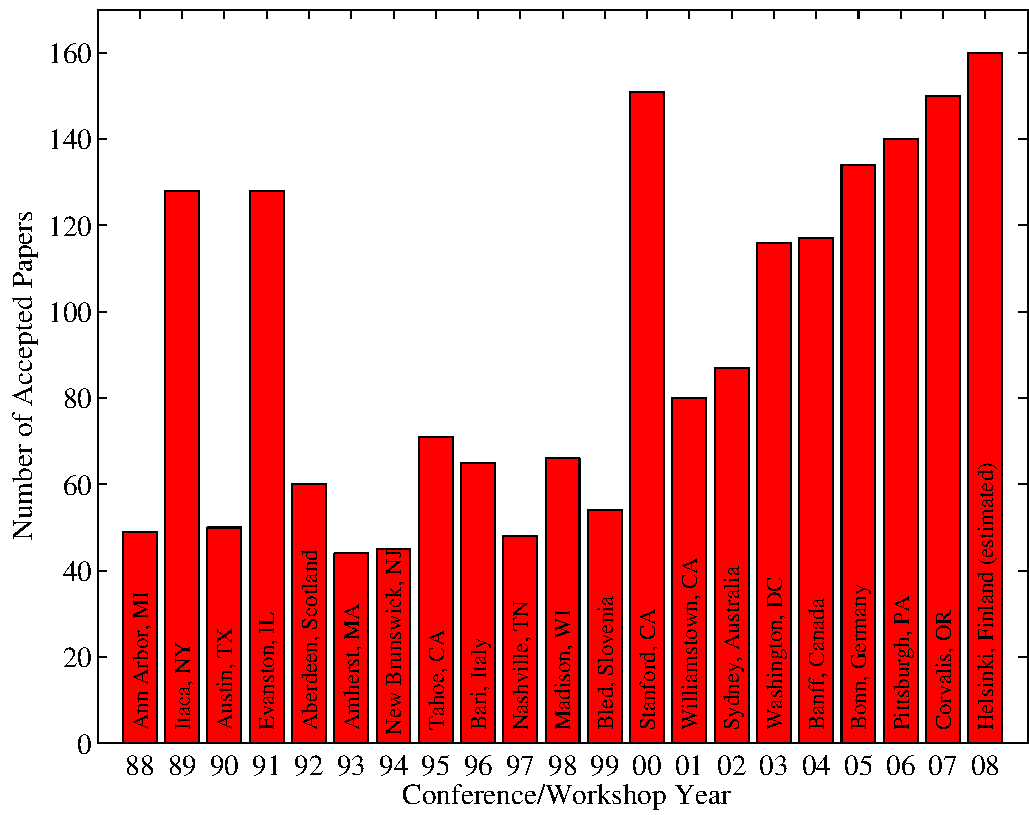
\includegraphics[width=\columnwidth]{icml_numpapers}}
\caption{Historical locations and number of accepted papers for International
Machine Learning Conferences (ICML 1993 -- ICML 2008) and International
Workshops on Machine Learning (ML 1988 -- ML 1992). At the time this figure was
produced, the number of accepted papers for ICML 2008 was unknown and instead
estimated.}
\label{icml-historical}
\end{center}
\vskip -0.2in
\end{figure}

\subsection{Figures}

You may want to include figures in the paper to illustrate
your approach and results. Such artwork should be centered,
legible, and separated from the text. Lines should be dark and at
least 0.5~points thick for purposes of reproduction, and text should
not appear on a gray background.

Label all distinct components of each figure. If the figure takes the
form of a graph, then give a name for each axis and include a legend
that briefly describes each curve. Do not include a title inside the
figure; instead, the caption should serve this function.

Number figures sequentially, placing the figure number and caption
\emph{after} the graphics, with at least 0.1~inches of space before
the caption and 0.1~inches after it, as in
Figure~\ref{icml-historical}. The figure caption should be set in
9~point type and centered unless it runs two or more lines, in which
case it should be flush left. You may float figures to the top or
bottom of a column, and you may set wide figures across both columns
(use the environment \texttt{figure*} in \LaTeX). Always place
two-column figures at the top or bottom of the page.

\subsection{Algorithms}

If you are using \LaTeX, please use the ``algorithm'' and ``algorithmic''
environments to format pseudocode. These require
the corresponding stylefiles, algorithm.sty and
algorithmic.sty, which are supplied with this package.
Algorithm~\ref{alg:example} shows an example.

\begin{algorithm}[tb]
   \caption{Bubble Sort}
   \label{alg:example}
\begin{algorithmic}
   \STATE {\bfseries Input:} data $x_i$, size $m$
   \REPEAT
   \STATE Initialize $noChange = true$.
   \FOR{$i=1$ {\bfseries to} $m-1$}
   \IF{$x_i > x_{i+1}$}
   \STATE Swap $x_i$ and $x_{i+1}$
   \STATE $noChange = false$
   \ENDIF
   \ENDFOR
   \UNTIL{$noChange$ is $true$}
\end{algorithmic}
\end{algorithm}

\subsection{Tables}

You may also want to include tables that summarize material. Like
figures, these should be centered, legible, and numbered consecutively.
However, place the title \emph{above} the table with at least
0.1~inches of space before the title and the same after it, as in
Table~\ref{sample-table}. The table title should be set in 9~point
type and centered unless it runs two or more lines, in which case it
should be flush left.

% Note use of \abovespace and \belowspace to get reasonable spacing
% above and below tabular lines.

\begin{table}[t]
\caption{Classification accuracies for naive Bayes and flexible
Bayes on various data sets.}
\label{sample-table}
\vskip 0.15in
\begin{center}
\begin{small}
\begin{sc}
\begin{tabular}{lcccr}
\toprule
Data set & Naive & Flexible & Better? \\
\midrule
Breast    & 95.9$\pm$ 0.2& 96.7$\pm$ 0.2& $\surd$ \\
Cleveland & 83.3$\pm$ 0.6& 80.0$\pm$ 0.6& $\times$\\
Glass2    & 61.9$\pm$ 1.4& 83.8$\pm$ 0.7& $\surd$ \\
Credit    & 74.8$\pm$ 0.5& 78.3$\pm$ 0.6&         \\
Horse     & 73.3$\pm$ 0.9& 69.7$\pm$ 1.0& $\times$\\
Meta      & 67.1$\pm$ 0.6& 76.5$\pm$ 0.5& $\surd$ \\
Pima      & 75.1$\pm$ 0.6& 73.9$\pm$ 0.5&         \\
Vehicle   & 44.9$\pm$ 0.6& 61.5$\pm$ 0.4& $\surd$ \\
\bottomrule
\end{tabular}
\end{sc}
\end{small}
\end{center}
\vskip -0.1in
\end{table}

Tables contain textual material, whereas figures contain graphical material.
Specify the contents of each row and column in the table's topmost
row. Again, you may float tables to a column's top or bottom, and set
wide tables across both columns. Place two-column tables at the
top or bottom of the page.

\subsection{Citations and References}

Please use APA reference format regardless of your formatter
or word processor. If you rely on the \LaTeX\/ bibliographic
facility, use \texttt{natbib.sty} and \texttt{icml2019.bst}
included in the style-file package to obtain this format.

Citations within the text should include the authors' last names and
year. If the authors' names are included in the sentence, place only
the year in parentheses, for example when referencing Arthur Samuel's
pioneering work \yrcite{Samuel59}. Otherwise place the entire
reference in parentheses with the authors and year separated by a
comma \cite{Samuel59}. List multiple references separated by
semicolons \cite{kearns89,Samuel59,mitchell80}. Use the `et~al.'
construct only for citations with three or more authors or after
listing all authors to a publication in an earlier reference \cite{MachineLearningI}.

Authors should cite their own work in the third person
in the initial version of their paper submitted for blind review.
Please refer to Section~\ref{author info} for detailed instructions on how to
cite your own papers.

Use an unnumbered first-level section heading for the references, and use a
hanging indent style, with the first line of the reference flush against the
left margin and subsequent lines indented by 10 points. The references at the
end of this document give examples for journal articles \cite{Samuel59},
conference publications \cite{langley00}, book chapters \cite{Newell81}, books
\cite{DudaHart2nd}, edited volumes \cite{MachineLearningI}, technical reports
\cite{mitchell80}, and dissertations \cite{kearns89}.

Alphabetize references by the surnames of the first authors, with
single author entries preceding multiple author entries. Order
references for the same authors by year of publication, with the
earliest first. Make sure that each reference includes all relevant
information (e.g., page numbers).

Please put some effort into making references complete, presentable, and
consistent. If using bibtex, please protect capital letters of names and
abbreviations in titles, for example, use \{B\}ayesian or \{L\}ipschitz
in your .bib file.

\subsection{Software and Data}

We strongly encourage the publication of software and data with the
camera-ready version of the paper whenever appropriate. This can be
done by including a URL in the camera-ready copy. However, do not
include URLs that reveal your institution or identity in your
submission for review. Instead, provide an anonymous URL or upload
the material as ``Supplementary Material'' into the CMT reviewing
system. Note that reviewers are not required to look at this material
when writing their review.

% Acknowledgements should only appear in the accepted version.
\section*{Acknowledgements}

\textbf{Do not} include acknowledgements in the initial version of
the paper submitted for blind review.

If a paper is accepted, the final camera-ready version can (and
probably should) include acknowledgements. In this case, please
place such acknowledgements in an unnumbered section at the
end of the paper. Typically, this will include thanks to reviewers
who gave useful comments, to colleagues who contributed to the ideas,
and to funding agencies and corporate sponsors that provided financial
support.


% In the unusual situation where you want a paper to appear in the
% references without citing it in the main text, use \nocite
\nocite{langley00}

\bibliography{example_paper}
\bibliographystyle{icml2019}


%%%%%%%%%%%%%%%%%%%%%%%%%%%%%%%%%%%%%%%%%%%%%%%%%%%%%%%%%%%%%%%%%%%%%%%%%%%%%%%
%%%%%%%%%%%%%%%%%%%%%%%%%%%%%%%%%%%%%%%%%%%%%%%%%%%%%%%%%%%%%%%%%%%%%%%%%%%%%%%
% DELETE THIS PART. DO NOT PLACE CONTENT AFTER THE REFERENCES!
%%%%%%%%%%%%%%%%%%%%%%%%%%%%%%%%%%%%%%%%%%%%%%%%%%%%%%%%%%%%%%%%%%%%%%%%%%%%%%%
%%%%%%%%%%%%%%%%%%%%%%%%%%%%%%%%%%%%%%%%%%%%%%%%%%%%%%%%%%%%%%%%%%%%%%%%%%%%%%%
\appendix
\section{Do \emph{not} have an appendix here}

\textbf{\emph{Do not put content after the references.}}
%
Put anything that you might normally include after the references in a separate
supplementary file.

We recommend that you build supplementary material in a separate document.
If you must create one PDF and cut it up, please be careful to use a tool that
doesn't alter the margins, and that doesn't aggressively rewrite the PDF file.
pdftk usually works fine. 

\textbf{Please do not use Apple's preview to cut off supplementary material.} In
previous years it has altered margins, and created headaches at the camera-ready
stage. 
%%%%%%%%%%%%%%%%%%%%%%%%%%%%%%%%%%%%%%%%%%%%%%%%%%%%%%%%%%%%%%%%%%%%%%%%%%%%%%%
%%%%%%%%%%%%%%%%%%%%%%%%%%%%%%%%%%%%%%%%%%%%%%%%%%%%%%%%%%%%%%%%%%%%%%%%%%%%%%%


\end{document}


% This document was modified from the file originally made available by
% Pat Langley and Andrea Danyluk for ICML-2K. This version was created
% by Iain Murray in 2018, and modified by Alexandre Bouchard in
% 2019. Previous contributors include Dan Roy, Lise Getoor and Tobias
% Scheffer, which was slightly modified from the 2010 version by
% Thorsten Joachims & Johannes Fuernkranz, slightly modified from the
% 2009 version by Kiri Wagstaff and Sam Roweis's 2008 version, which is
% slightly modified from Prasad Tadepalli's 2007 version which is a
% lightly changed version of the previous year's version by Andrew
% Moore, which was in turn edited from those of Kristian Kersting and
% Codrina Lauth. Alex Smola contributed to the algorithmic style files.
